\newgeometry{margin=85pt}
\chapter*{Sistema de Referencia de Coordenadas}
\setcounter{chapter}{3} 
\setcounter{section}{0}
\addcontentsline{toc}{chapter}{Sistema de Referencia de Coordenadas}

Un Sistema de Referencia de Coordenadas (SRC) o \textit{Coordinate Reference System} (CRS), es un sistema que determina unívocamente la posición de cualquier punto de la superficie terrestre, 
lo cual constituye una de las principales características de los GIS.
Para ello, se emplean tuplas de 3 números denominados coordenadas, estas pueden ser geográficas (latitud, longitud, altura) o proyectadas (X, Y, Z).
Según el tipo de coordenadas, tenemos dos sistemas de referencia: Sistema de coordenadas geográficas y sistema de coordenadas proyectadas.

\section{Sistema de coordenadas geográficas}
Un Sistema de Coordenadas Geográficas (SCG) o \textit{Geographic Coordinate System} (GCS), utiliza la superficie esférica tridimensional de La Tierra para definir lugares reales de la misma.
Se apoya en los Polos y en el Ecuador para construir una red geográfica, formada por paralelos y meridianos.

\begin{figure}[H]
  \centering
  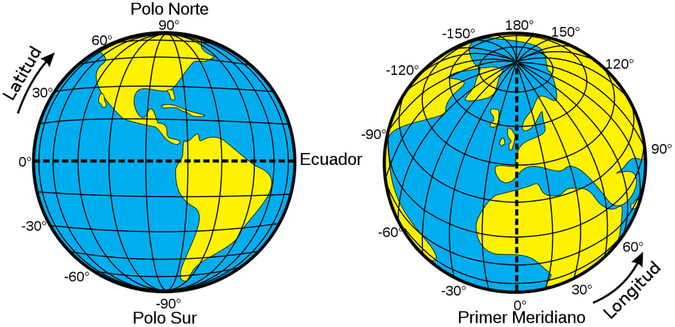
\includegraphics[width=0.55\textwidth]{Imagenes/CRS/GCS.png}
  \caption{Proyecciones ortográficas de la Tierra con paralelos y meridianos} \label{fig:GCS}
\end{figure}

La figura \ref{fig:GCS} muestra dos proyecciones distintas del GCS. 
En ambas, las líneas horizontales o paralelos presentan el mismo valor de latitud, y las líneas verticales o meridianos presentan el mismo valor de longitud. 
El globo terráqueo de la izquierda corresponde a una proyección ecuatorial, en la que podemos observar algunos valores de latitud. 
El ecuador es el paralelo 0° y divide el globo en hemisferios norte y sur, teniendo el polo norte una latitud 90° N y el polo sur una latitud 90° S.
A la derecha se observa una proyección oblicua, en la que se muestran algunos valores de la longitud. Podemos observar que a partir de un meridiano base se miden las longitudes.
Para la mayoría de los GCS, el meridiano base es la longitud que atraviesa Greenwich, situado al sureste de Londres. 
Entonces, el Primer Meridiano es el meridiano 0° y los siguientes meridianos se miden desde 0 hasta 180 grados al este o al oeste del primer meridiano.
Los valores de longitud hacia el oeste del primer meridiano tienen valores negativos, para su uso en aplicaciones de cartografía digital.

Para hacer referencia a un punto en la superficie de La Tierra, se utilizan sus valores de latitud, longitud y altitud.
\begin{itemize}
  \item La latitud es el ángulo entre el plano ecuatorial y la línea que pasa por el punto y el centro de la Tierra. 
  \item La longitud es el ángulo entre el meridiano de referencia y el meridiano que pasa por el punto.
  \item La altitud es la distancia vertical que existe entre cualquier punto de la Tierra en relación al nivel del mar.
\end{itemize}

Existen diferentes formatos y notaciones para definir las coordenadas, las cuales se exponen en la siguiente tabla:
\renewcommand{\arraystretch}{2}
\begin{table}[h!]
  \tiny
  \centering
      \begin{tabular}{|c|c|c|c|} 
      \hline
      Notación & Latitud & Longitud & Ejemplo \\  \hline
      \multirow{2}{*}{
        \centering %        
        \parbox{10em}{\hspace{1cm}DD\\(Grados decimales)}} & [ + $|$ - ] DD,dddd & [ + $|$ - ] DDD,dddd & 40.76, -73.984 \\ \cline{2-4} 
                               & DD,dddd [ N $|$ S ] & DDD,dddd [ E $|$ O ] & 40.76 N, 73.984 O \\ \hline
      \multirow{2}{*}{
        \centering %
        \parbox{10em}{\vspace{1mm}\hspace{0.9cm}DM\\(Grados:Minutos)\\}} & [ + $|$ - ] DD° MM.mmm’ & [ + $|$ - ] DDD° MM.mmm’ & 40° 45.6’ , -73° 59.04’ \\ \cline{2-4} 
                               & DD° MM.mmm’ [ N $|$ S ] & DDD° MM.mmm’ [ E $|$ O ] & 40° 45.6’ N, 73° 59.04’ O \\ \hline
      \multirow{2}{*}{
        \centering %
        \parbox{12em}{\vspace{1mm}\hspace{1.2cm}DMS\\(Grados:Minutos:Segundos)\\}} & [ + $|$ - ] DD° MM’ SS,sss’’ & [ + $|$ - ] DDD° MM’ SS,sss’’ & 40° 45’ 36’’, -73° 59’ 2.4’’ \\ \cline{2-4} 
                                & [ N $|$ S ] DD° MM’ SS,sss’’ & [ E $|$ O ] DD° MM’ SS,sss’’ & 40° 45’ 36’’ N, 73° 59’ 2.4’’ O \\ \hline
  \end{tabular}
  \caption{Tipos de notaciones de coordenadas}
  \label{tabla:coordFormats}
\end{table}  
\renewcommand{\arraystretch}{1}

En la tabla \ref{tabla:coordFormats} el grado-signo puede ir delante o detrás del valor de la coordenada.

\section{Sistema de coordenadas proyectadas}

A diferencia de los GCS, los Sistema de Coordenadas Proyectadas (SCP) o \textit{Projected Coordinate System} (PCS),
localizan ubicaciones en una superficie plana de La Tierra a través de proyecciones cartográficas,
las cuales crean una representación métrica bidimensional de la superficie tridimensional de La Tierra.
Por lo tanto, las coordenadas de longitud y latitud pasan a ser coordenadas cartesianas (x e y), en un sistema con unidades métricas (pies, metros, kilómetros, pulgadas, etc.)
Estas representaciones planas de la esfera terrestre son más conocidas como mapas. Para su elaboración, los cartógrafos emplean distintos tipos de proyecciones cartográficas, agrupadas en tres familias principales, 
que resultan de rodear el globo terráqueo con superficies cilíndricas, cónicas o planas.

\begin{figure}[H]
  \centering
  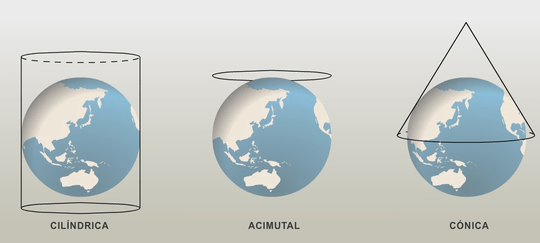
\includegraphics[width=0.60\textwidth]{Imagenes/CRS/proyecciones.png}
  \caption{Familias de proyecciones cartográficas de La Tierra} \label{fig:proyecciones}
\end{figure}

La figura \ref{fig:proyecciones} muestra los esquemas de los tres tipos de proyecciones cartográficas básicas: cilíndricas, cónicas y acimutales.

\subsection{Proyección cilíndrica}
Las proyecciones cilíndricas usan un cilindro tangente a la esfera terrestre, de tal manera que el cilindro contiene al globo terráqueo manteniendo el contacto con el Ecuador. 
La superficie terrestre se proyecta sobre el cilindro a partir de un foco de luz que se encuentra en el centro de La Tierra.

\begin{figure}[H]
  \centering
  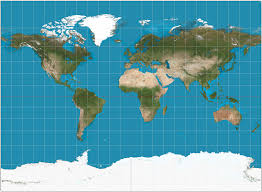
\includegraphics[width=0.50\textwidth]{Imagenes/CRS/proyeccion-cilindrica.png}
  \caption{Mapa proyección cilíndrica} \label{fig:proyeccion-cilindrica}
\end{figure}

La figura \ref{fig:proyeccion-cilindrica} muestra el mapa resultante de la proyección cilíndrica, el cuál presenta una red de paralelos y meridianos perpendiculares.
La deformación de la escala es proporcional a la distancia con el Ecuador, donde se conserva la escala.
A pesar de esta deformación, está representación resulta útil en ciertos campos como el de la navegación, debido principalmente a la sencillez que aporta la perpendicularidad entre meridianos y paralelos.
Es una de las proyecciones más utilizadas, aunque por lo general en forma modificada, debido a las grandes distorsiones que ofrece en las zonas de latitud elevada, lo que impide apreciar a las regiones polares en su verdadera proporción. 

\subsection{Proyección cónica}
Las proyecciones cónicas usan un cono tangente a la esfera terrestre, situando el vértice en el eje que une los dos polos, de tal manera que el cono se sitúa encima de La Tierra. 
La superficie terrestre se proyecta sobre el cono a partir de un foco de luz situado en el vértice del mismo, es decir, en uno de los dos polos.

\begin{figure}[H]
  \centering
  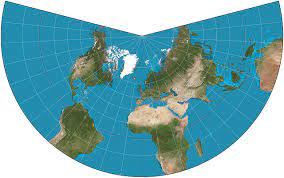
\includegraphics[width=0.50\textwidth]{Imagenes/CRS/proyeccion-conica.png}
  \caption{Mapa proyección cónica} \label{fig:proyeccion-conica}
\end{figure}

La figura \ref{fig:proyeccion-conica} muestra el mapa resultante de la proyección cónica, el cuál presenta los meridianos como líneas rectas que parten del polo,
mientras que los paralelos son circunferencias concéntricas con centro el polo.
Los paralelos o paralelo que mantienen el contacto con el cono, se denominan paralelos de referencia, y en ellos se conserva la escala, aumentando la deformación a medida que nos alejamos.
Por lo tanto, esta representación resulta útil para aquellos países que se encuentran en las regiones de latitudes medias.

\subsection{Proyección acimutal}
Las proyecciones acimutales usan un plano tangente a un punto de la superficie terrestre, pero pueden reproducirse con diferentes perspectivas según dónde situemos el foco de luz.
En la proyección acimutal gnomónica, el foco de luz se sitúa en el centro de La Tierra, en la estereográfica, en el polo opuesto del globo, y en la ortográfica, en un punto del espacio exterior.
En todas las perspectivas no se proyecta toda la superficie de La Tierra, sino que se proyecta una porción de la misma.

\begin{figure}[H]
  \centering
  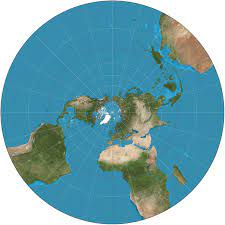
\includegraphics[width=0.50\textwidth]{Imagenes/CRS/proyeccion-acimutal.png}
  \caption{Mapa proyección acimutal} \label{fig:proyeccion-acimutal}
\end{figure}

La figura \ref{fig:proyeccion-acimutal} muestra el mapa resultante de la proyección acimutal, el cuál presenta las mismas características que el mapa de la proyección cónica en cuanto a meridianos y paralelos, pero en este caso el centro es el punto tangencial a la esfera terrestre, dando lugar a un mapa con forma circular.
En cuanto a la distorsión que provocan, se obtiene una mayor distorsión cuanto mayor sea la distancia al foco de luz. 
A diferencia de las proyecciones cónicas y cilíndricas, la distorsión aumenta en el Ecuador, por lo tanto, esta representación resulta útil para representar los polos.
\\
\\

\begin{figure}[H]
  \centering
  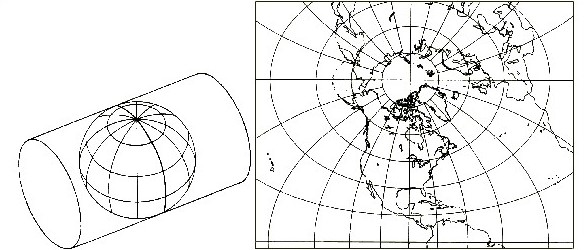
\includegraphics[width=0.60\textwidth]{Imagenes/CRS/utm.jpg}
  \caption{Proyección universal transversal de Mercator} \label{fig:UTM}
\end{figure}
Por cada familia, existen diversos tipos de proyecciones, en las cuales no vamos a profundizar. Pero sí que resulta interesante comentar algunos ejemplos de las proyecciones más conocidas y utilizadas.
Entre las proyecciones cartográficas destaca la proyección cilíndrica de Mercator, ideada por Gerardus Mercator en 1569, la cuál revolucionó la cartografía. 
El sistema de coordenadas universal transversal de Mercator o \textit{Universal Transverse Mercator} (UTM), es un PCS basado en esta proyección, 
pero en vez de hacerla tangente al Ecuador (Mercator normal), se la hace secante a un meridiano, tal y como se observa en la figura \ref{fig:UTM}
UTM es la proyección mundial, por lo que podemos representar cualquier parte del mundo con ella.
Como en el resto de proyecciones cilíndricas, los meridianos y paralelos son líneas rectas paralelas entre sí. Además en la proyección de Mercator, los meridianos son equidistantes y se extienden hacia el infinito al acercarse a los polos.
Esta representación resulta útil para realizar cartas náuticas, debido a que las líneas rectas representan rumbos reales de la brújula.
La variante Web Mercator es la proyección estándar para los servicios web de mapas, la cuál esta disponible en la mayoría entornos GIS del mercado, así como distintas versiones de esta proyección.

Otra de las proyecciones más usadas y populares es la proyección cónica de Lambert, llamada así por su creador Johann Heinrich Lambert. 
En ella, los meridianos son líneas rectas cuyo origen es el vértice del cono, y los paralelos son circunferencias concéntricas respecto al vértice del cono.
Esta representación fue usada principalmente en los mapas militares, debido a que la distorsión es mínima en una gran extensión del terreno, siendo nula en los paralelos de referencia.

La mayor diferencia con los GCS es que los PCS presentan mayor facilidad para trabajar, pero las distancias y ángulos presentan mayor distorsión debido a la proyección.
Los GCS permiten ubicar mejor las posiciones, en cambio los PCS son mejores para medir distancias o calcular áreas de los objetos.

\section{Datums Geodésicos}
% https://www.aristasur.com/sites/as/users/3/arch/datum-cartografia.pdf

El datum de un dato geográfico se define mediante un sistema de referencia y una proyección cartográfica.
Por ejemplo, podemos tener como sistema de referencia el WGS84, el cual veremos a continuación, y como proyección la proyección cónica de Lambert.
Su objetivo es describir la forma y el tamaño de La Tierra más acorde a la realidad.
Como hemos visto, los CRS representan la superficie de La Tierra, pero lo realizan con ciertas irregularidades debido a que esta no presenta una forma esférica perfecta.

\subsection{Elipsoide}

\begin{figure}[H]
  \centering
  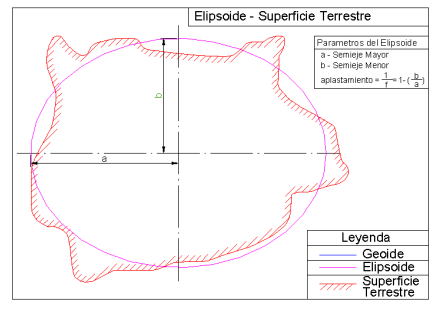
\includegraphics[width=0.60\textwidth]{Imagenes/CRS/esferoide.png}
  \caption{Comparación entre la superficie y el esferoide terrestre} \label{fig:esferoide}
\end{figure}

Un Esferoide (o Elipsoide) representa La Tierra con mayor precisión, y surge como resultado de achatar la esfera terrestre por los polos, tal y como podemos observar en la figura \ref{fig:esferoide}.
Un Esferoide queda definido por su semieje mayor (a), y su semieje menor (b), o por (a) y su aplastamiento (f), obtenido de la siguiente manera:
\begin{equation}
  f = \frac{(a-b)}{a} \Leftrightarrow \frac{1}{f} = 1 - (\frac{b}{a})
\end{equation}
En el caso del esferoide terrestre, tenemos que el semieje a corresponde al Radio Ecuatorial y el semieje b al Radio Polar.

Hayford propuso en 1924 en la Asamblea Internacional de Geodesia y Geofísica (Madrid) un Elipsoide Internacional de Referencia, 
con un Radio Ecuatorial de 6378388 metros y un aplastamiento de 297 metros.
Este elipsoide fue utilizado ampliamente por la mayoría de países, no siendo perfeccionado hasta 1964,
donde la Unión Astronómica Internacional en Hamburgo estableció unos nuevos valores de 6378160 metros de Radio Ecuatorial y 298,25 metros de aplastamiento.
Finalmente, se adoptó el Sistema de Referencia Geodésico 1980 o \textit{Geodetic Reference System 1980} (GRS80) por la Asamblea General de Asociación Internacional de Geodesia (IAG) del año 1979.
El GRS80 presenta un Radio Ecuatorial de 6378137 metros y un aplastamiento de 298.257222101 metros. 

\subsection{Geoide}

Para definir completamente el término de Datum Geodésico, también es necesario introducir el concepto de Geoide.
El Geoide se define como la superficie teórica de La Tierra que une todos los puntos que presentan una atracción gravitatoria constante. 

\begin{figure}[H]
  \centering
  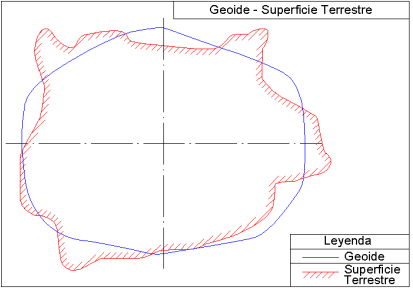
\includegraphics[width=0.60\textwidth]{Imagenes/CRS/geoide.png}
  \caption{Comparación entre la superficie y el geoide terrestre} \label{fig:geoide}
\end{figure}

Aunque no lo parezca, esta superficie no es uniforme, debido a la distinta composición mineral y densidad del interior de La Tierra,
provoca que exista una distancia distinta desde el centro de La Tierra al punto del Geoide, tal y como podemos ver en la figura \ref{fig:geoide}. 
Dichas variaciones de densidad provocan anomalías gravimétricas que ocasionan la superficie irregular de Geoide.
Tanto la figura \ref{fig:esferoide} como la figura \ref{fig:geoide} se han obtenido del estudio \cite{DATUM}.

El Geoide resulta más específico que el elipsoide a la hora de definir la forma de La Tierra. 
Aunque la diferencia máxima entre las superficies de ambas representaciones está en el orden de 100 metros. Estas diferencias se conocen como alturas geoidales.

Al igual que en el caso de los elipsoides, existen diversos geoides de referencia, y estos no son constantes en el tiempo,
sino que evolucionan para adaptarse a las modificaciones que tienen lugar sobre la superficie terrestre.

\subsection{Punto fundamental}

Los datum globales son los que se utilizan para georreferenciar cualquier punto de la superficie de La Tierra, así que, tanto el centro del elipsoide, como su plano ecuatorial, deben coincidir con los terrestres.
También existen los datums locales, que tratan de adaptar mejor el CRS a la superficie terrestre perteneciente a una región concreta.
Para estos últimos, necesitamos ubicar el elipsoide en un punto de la superficie de La Tierra.
Por lo tanto, cada datum local, además de por el modelo asociado de la forma de La Tierra (elipsoide) y por un modelo de campo de gravedad (geoide), está compuesto por un punto de referencia de la superficie de La Tierra,
denominado punto fundamental. En este punto, el elipsoide es tangente al geoide y la distancia desde el centro de La Tierra es la misma para ambas formas geométricas.
El punto fundamental queda definido por sus coordenadas geográficas (Latitud y Longitud). 

Para un mismo elipsoide pueden utilizarse distintos puntos fundamentales, que darán lugar a distintos datums, y por lo tanto, a distintas coordenadas para un mismo punto.

\subsection{Ejemplos}
En el caso de la España, en 1970 se adoptó el Datum Europeo 1950 o \textit{European Datum 1950} (ED50) como sistema geodésico oficial.
El ED50 tiene como Elipsoide la propuesta por Hayford en 1924 y como punto de referencia Postman (Alemania), cuyas coordenadas geográficas son 52° 22’ 51.446’’ O, 13° 03’ 58.741’’ E.
Actualmente, el Real Decreto \cite{BOE2007} establece el Sistema Europeo de Referencia Terrestre 1989 o \textit{European Terrestrial Reference System 1989} (ETRS89), 
como sistema de referencia geodésico oficial en España, exceptuando las Islas Canarias que adoptan la Red Geodésica Nacional por Técnicas Espaciales Canarias 1995 (REGCAN95).
Ambos sistemas tienen asociado el elipsoide GRS80.
  
En cuanto al datum global, el Sistema Geodésico Mundial 1984 o \textit{World Geodetic System 1984} (WGS84), es el sistema de coordenadas geográficas usado mundialmente desde 1984.
El WGS84 es utilizado habitualmente en la comunidad GIS y el datum por defecto en todos los dispositivos GPS. 
La elipsoide WGS84 es semejante a la elipsoide GRS80, siendo esta última un poco más aplanada.

\section{Identificador de Referencia Espacial}

El Identificador de Sistemas de Referencia Espacial o \textit{Spatial Reference System Identifier} (SRID), es un código que identifica de forma unívoca los sistemas de coordenadas.
Actualmente, el SRID se conoce como EPSG, acrónimo de \textit{European Petroleum Survey Group}, organización relacionada con la industria petrolera en Europa, debido a que este organismo 
desarrolló y difundió el conjunto de parámetros geodésicos EPSG, un repositorio con elipsoides, datums, sistemas de coordenadas, proyecciones cartográficas, etc.
Podemos consultar los códigos EPSG / SRID accediendo a la dirección \cite{EPSG-SRID-codes}.
Por ejemplo, el código 4326 corresponde al sistema de coordenadas WGS84 y el código 3857 a la variante Web Mercator.
\\
\\
Para finalizar, es importante destacar que ningún CRS es perfecto, todo CRS implica una compensación que puede distorsionar tanto forma, distancia o/y área de los datos reales.

\section{Transformación y conversión de coordenadas}
Cada proveedor de datos geográficos genera información con un datum determinado, es decir, con un sistema de referencia y una proyección cartográfica concretos.
La realidad es que estos proveedores no se adaptan a las necesidades de cada particular,
por lo tanto necesitamos transformar los distintos datums en el datum que mejor se ajuste a nuestra representación.
Para tener único sistema de referencia y una única proyección es necesario realizar distintas operaciones, de las cuales nos distinguimos dos tipos:
\begin{itemize}
  \item Conversión de coordenadas\\
  Los sistemas de origen y destino comparten el mismo sistema de referencia.  
  Es una transformación exacta y se basa en la aplicación de formulas establecidas que relacionan ambos sistemas.
  Por ejemplo, tengo un datum con un sistema de referencia WGS84 y una proyección de Lambert, 
  y aplicamos una conversión para que el datum resultante sea con una proyección UTM, manteniendo el mismo sistema de referencia. 
  \item Transformación de coordenadas\\
  El sistema de referencia es distinto en los sistemas de origen y destino. 
  Por ejemplo, tenemos un mapa con un sistema WGS84 y otro mapa con un sistema ETRS89, ambos con una proyección UTM.
  Entonces, para llegar del uno al otro se requiere una transformación del sistema de referencia.
\end{itemize}

Existen distintas herramientas que nos permitan realizar estas operaciones, por ejemplo, el Instituto Geográfico Nacional (IGN), mediante el programa de aplicaciones geodésicas (PAG),
ofrece una calculadora geodésica que permite transformaciones entre coordenadas geográficas o entre datums.





